

\begin{frame}[t,allowframebreaks]{
    Beyond the gradient: The Hessian matrix -}

    Often, we are interested to know {\bf how the 
    \underline{first derivative} of a 
    function will change as we vary the input} of the function.\\
    \begin{itemize}
        \item
        Naturally, this information is described by the 
        \underline{second derivative} of the function 
        (ie. the derivative of the derivative).\\
    \end{itemize}

    \vspace{0.2cm}

    The second derivative of a function is {\bf a measure of its curvature}.\\

    \begin{columns}
        \begin{column}{0.42\textwidth}
        
            The curvature determines

        \end{column}
        \begin{column}{0.58\textwidth}

            \begin{center}
                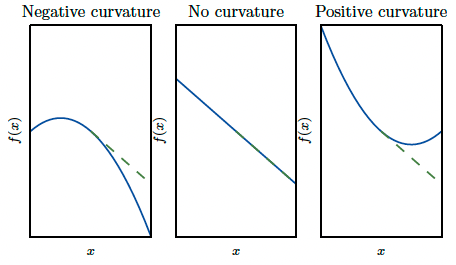
\includegraphics[width=1.00\textwidth]
                    {./images/grad_descent/goodfellow17_curvature_1d.png}\\
                {\tiny 
                    \color{col:attribution} 
                    Schematic reproduced from p. 84 of \cite{Goodfellow:2017MITDL}.\\
                }
            \end{center}        
        
        \end{column}
    \end{columns}

    \framebreak

    %
    %
   
    Suppose we have a function 
    $f(\vect{x})$: $\mathbb{R}^m \rightarrow \mathbb{R}$.
    The derivative wrt $x_i$ of the derivative of $f$ wrt to $x_j$ 
    is denoted by $\displaystyle \partial^2 f(\vect{x}) / \partial x_i \partial x_j$.\\        
    \vspace{0.1cm}

    These partial derivatives form the \gls{Hessian matrix} 
    $\vect{H}^{(f)}(\vect{x})$ with elements:
    \begin{equation}
        H^{(f)}_{ij}(\vect{x}) = 
        \frac{\partial^2 f(\vect{x})}{\partial x_i \partial x_j}
        \label{eq:hessian_1}
    \end{equation}\\
    
    Therefore:\\
    \vspace{-0.2cm}
    \begin{equation}
        \vect{H}^{(f)}(\vect{x}) = 
        % \left(
        %     \begin{array}{ccc}
        %         \frac{\partial \vect{f}(\vect{x})}{\partial x_1} & 
        %         \cdots & 
        %         \frac{\partial \vect{f}(\vect{x})}{\partial x_n} \\ 
        %     \end{array}
        % \right) =
        % \left(
        %     \begin{array}{c}
        %         \nabla_{\vect{x}}^T f_{1}(\vect{x}) \\
        %         \vdots \\
        %         \nabla_{\vect{x}}^T f_{m}(\vect{x}) \\
        %     \end{array}
        % \right) =
        \left(
            \begin{array}{cccc}
                \frac{\partial^2 f(\vect{x})}{\partial x_1^2} & 
                \frac{\partial^2 f(\vect{x})}{\partial x_1 \partial x_2} &
                \cdots & 
                \frac{\partial^2 f(\vect{x})}{\partial x_1 \partial x_m} \\ 
                \frac{\partial^2 f(\vect{x})}{\partial x_2 \partial x_1} & 
                \frac{\partial^2 f(\vect{x})}{\partial x_2^2} &
                \cdots & 
                \frac{\partial^2 f(\vect{x})}{\partial x_2 \partial x_m} \\ 
                \vdots &
                \vdots &
                \ddots & 
                \vdots \\
                \frac{\partial^2 f(\vect{x})}{\partial x_m \partial x_1} & 
                \frac{\partial^2 f(\vect{x})}{\partial x_m \partial x_2} & 
                \cdots & 
                \frac{\partial^2 f(\vect{x})}{\partial x_m^2} \\ 
            \end{array}
        \right)
        \label{eq:hessian_2}
    \end{equation}\\
    
    \vspace{0.25cm}

    \index{Hessian matrix}\index{Jacobian matrix}
    Note that {\bf the \gls{Hessian} is the \gls{Jacobian} of the gradient}.

    \framebreak

    %
    %

    \begin{itemize}
        \item 
        Anywhere the second-order partial derivatives are continuous,
        the \gls{Hessian matrix} is {\bf symmetric}:
        \begin{equation}
            H^{(f)}_{ij}(\vect{x}) = 
              \frac{\partial^2 f(\vect{x})}{\partial x_i \partial x_j} =
              \frac{\partial^2 f(\vect{x})}{\partial x_j \partial x_i} =
              H^{(f)}_{ji}(\vect{x}) 
            \label{eq:hessian_symmetric_1}
         \end{equation}\\
         \begin{equation}
              \vect{H}^{(f)}(\vect{x}) = \Big( \vect{H}^{(f)}(\vect{x}) \Big)^T
            \label{eq:hessian_symmetric_2}
         \end{equation}\\
    
        \item 
        Because $\vect{H}^{(f)}(\vect{x})$ is real and symmetric,
        it can be decomposed into a set of real 
        \index{eigenvalue}\glspl{eigenvalue} $\lambda_{i}$
        and an orthogonal basis of 
        \index{eigenvector}\glspl{eigenvector} $\vect{\hat{e}}_i$.
        $\vect{H}^{(f)}(\vect{x})$ is {\bf diagonalizable} and
        there exist a matrix $\vect{O}$ such that:
        \begin{equation}
            \vect{H}^{(f)}(\vect{x}) = 
            \vect{O}
            \left(
                \begin{array}{ccc}
                    \lambda_1 &        & \\
                              & \ddots & \\
                              &        & \lambda_m \\                              
                \end{array}
            \right)
            \vect{O}^{-1}
          \label{eq:hessian_diag_1}
       \end{equation}\\
    \end{itemize}

    \framebreak

    %
    %

    \begin{itemize}
        \item 
        The second derivative in a particular direction
        expressed by a unit vector $\vect{\hat{u}}$ is given by
        $\displaystyle \vect{\hat{u}}^T \cdot \vect{H}^{(f)}(\vect{x}) \cdot \vect{\hat{u}}$.
        \begin{itemize}
            \item If $\vect{\hat{u}}$ is one of the 
            \index{eigenvector}\glspl{eigenvector}, $\vect{\hat{e}}_i$,
            {\bf the corresponding 
            \index{eigenvalue}\gls{eigenvalue} gives the second-order 
            derivative in that direction}.
            \item In all other directions, the directional 
            {\bf second-order derivative is 
            a weighted average of all \glspl{eigenvalue} $\lambda_{i}$}.
            \begin{itemize}
                \item All weights are between 0 and 1.
                \item Eigenvalues with larger weight correspond to \glspl{eigenvector}
                $\vect{\hat{e}}_i$ that are closer to the direction of $\vect{\hat{u}}$.
            \end{itemize}
            \item The minimum (maximum) \gls{eigenvalue} determined the minimum (maximum)
            directional second-order derivative.
        \end{itemize}
    
    \end{itemize}

    \framebreak

    %
    %

    Using a second-order \index{Taylor series}\gls{Taylor series}, we can approximate 
    the value of the function $f$ at $\vect{x}^\prime$, 
    a small distance away from $\vect{x}$:
    \vspace{-0.1cm}
    \begin{equation}
        f(\vect{x}^\prime) \approx 
          f(\vect{x}) + 
          (\vect{x}^\prime - \vect{x})^T \cdot \nabla_{\vect{x}}f(\vect{x}) +
          \frac{1}{2} (\vect{x}^\prime - \vect{x})^T \cdot 
            \vect{H}^{(f)}(\vect{x}) \cdot (\vect{x}^\prime - \vect{x})
        \label{eq:hessian_taylor_1}
    \end{equation}

    If $\alpha$ is the \index{learning rate}\gls{learning rate}, 
    the gradient-based optimization procedure moves from point $\vect{x}$ 
    to the point $\vect{x}^\prime$ given by Eq.~\ref{eq:grad_descent_1}
    ($\displaystyle \vect{x}^\prime = \vect{x} - \alpha \nabla_{\vect{x}}f(\vect{x})$).\\
    \vspace{0.2cm}

    Substituting Eq.~\ref{eq:grad_descent_1} into Eq.~\ref{eq:hessian_taylor_1}, 
    we obtain:
    \vspace{-0.1cm}
    \begin{equation}
        f(\vect{x}^\prime) \approx 
        f(\vect{x}) 
        {\color{cadmiumgreen}
          - \alpha 
           \nabla_{\vect{x}}^{T}f(\vect{x}) \cdot 
           \nabla_{\vect{x}}f(\vect{x})      
        } 
        {\color{cadmiumred}      
           + \frac{1}{2} \alpha^2 
           \nabla_{\vect{x}}^{T}f(\vect{x}) \cdot 
           \vect{H}^{(f)}(\vect{x}) \cdot 
           \nabla_{\vect{x}}f(\vect{x})
        } 
        \label{eq:hessian_taylor_2}
    \end{equation}

    In Eq.~\ref{eq:hessian_taylor_2}, we recognize three terms describing:\\
    \begin{itemize}
        \item the original value of $f$,
        \item the {\color{cadmiumgreen}expected improvement due to the gradient of $f$}, and
        \item a {\color{cadmiumred}correction that accounts for the curvature of $f$}.
    \end{itemize}

    \framebreak

    %
    %

    The last term in Eq.~\ref{eq:hessian_taylor_2} is a
    {\color{cadmiumred}correction accounting for the curvature of $f$}.\\
    \vspace{-0.5cm}
    \begin{equation*}
        f(\vect{x}^\prime) \approx 
        f(\vect{x}) 
        {\color{cadmiumgreen}
          - \alpha 
           \nabla_{\vect{x}}^{T}f(\vect{x}) \cdot 
           \nabla_{\vect{x}}f(\vect{x})      
        } 
        {\color{cadmiumred}    
         \overbrace{  
           + \frac{1}{2} \alpha^2 
           \nabla_{\vect{x}}^{T}f(\vect{x}) \cdot 
           \vect{H}^{(f)}(\vect{x}) \cdot 
           \nabla_{\vect{x}}f(\vect{x})
         }^\text{$\delta_{curv}$}
        } 
    \end{equation*}

    Note that:
    \begin{itemize}
        \item 
        When $\delta_{curv} \le 0$, Eq.~\ref{eq:hessian_taylor_2} predicts that
        $f(\vect{x})$ will keep on decreasing for any value of $\alpha$,
        but the expansion will not remain accurate 
        for large $\alpha$.
        The optimal step size is found by trial and error.\\
        \item 
        When $\delta_{curv} > 0$, the optimal step size can be found by minimizing the 
        right-hand side of Eq.~\ref{eq:hessian_taylor_2} that is quadratic in $\alpha$:
        \begin{equation}
            \alpha_{opt} = 
            \frac{
                \nabla_{\vect{x}}^{T}f(\vect{x}) \cdot 
                \nabla_{\vect{x}}f(\vect{x})
            }{
                \nabla_{\vect{x}}^{T}f(\vect{x}) \cdot
                \vect{H}^{(f)}(\vect{x}) \cdot 
                \nabla_{\vect{x}}f(\vect{x})
            }
            \label{eq:taylor_optimum_step_1}     
        \end{equation}
        \item 
        If $\delta_{curv}$ is too large, 
        the \index{gradient descent}\gls{gradient descent} 
        step can move uphill!
    \end{itemize}

    \framebreak

    %
    %

    Using the 2$^{nd}$ derivative, $f^{\prime \prime}(x)$, we can determine whether a
    \index{critical point}\gls{critical point} (where $f^{\prime}(x)=0$) is a
    \index{local maximum}\gls{local maximum}, a
    \index{local minimum}\gls{local minimum}, or a
    \index{saddle point}\gls{saddle point}.\\        
    \vspace{-0.1cm}

    \begin{columns}
        \begin{column}{0.60\textwidth}        
            \begin{center}
                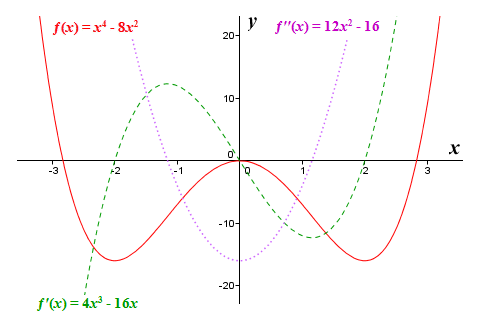
\includegraphics[width=1.00\textwidth]
                    {./images/grad_descent/techuk_second_derivative_test_1.png}\\
                {\tiny 
                    \color{col:attribution} 
                    Schematic reproduced from \cite{TechUK:2ndDerivativeTest}.\\
                }
            \end{center}        
        \end{column}
        \begin{column}{0.40\textwidth}
            \begin{itemize}
                \item If $f^{\prime \prime}(x) > 0$
            \end{itemize}
                
        \end{column}
    \end{columns}

    \vspace{0.1cm}
    In multiple dimensions, 
    we need to examine all the 2$^{nd}$-order derivatives
    of the function. The \index{Hessian matrix}\gls{Hessian matrix} supports this task.\\

    \framebreak

    %
    %

    The 2$^{nd}$ derivative test can be generalized in multiple dimensions
    using the \index{eigendecomposition}\gls{eigendecomposition} 
    of the \index{Hessian matrix}\gls{Hessian matrix}.\\
    \vspace{0.3cm}
    A \index{critical point}\gls{critical point},
    where $\nabla_{\vect{x}} f(\vect{x})=0$, is:
    \begin{itemize}
        \item 
        a \index{local minimum}\gls{local minimum}, 
        if the \gls{Hessian matrix} is 
        \index{positive definite}{\bf \gls{positive definite}}\\ 
        (i.e. all its \index{eigenvalue}\glspl{eigenvalue} are positive)
        \item 
        a \index{local maximum}\gls{local maximum}, 
        if the \gls{Hessian matrix} is 
        \index{negative definite}{\bf \gls{negative definite}}\\ 
        (i.e. all its \glspl{eigenvalue} are negative)
        \item 
        a \index{saddle point}\gls{saddle point}, 
        if at least one \gls{eigenvalue} is positive 
        and at least another one is negative.
    \end{itemize}

    \vspace{0.3cm}

    In multiple dimensions, the 2$^{nd}$ derivative 
    test can be {\bf inconclusive} 
    if at least one \gls{eigenvalue} is zero and 
    all nonzero \glspl{eigenvalue} have the same sign.

    \framebreak

    %
    %

    \begin{columns}
        \begin{column}{0.70\textwidth}        
            \begin{center}
                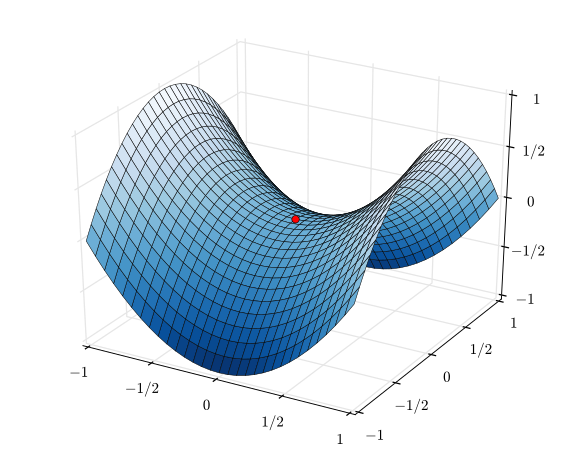
\includegraphics[width=1.00\textwidth]
                    {./images/grad_descent/wikipedia_saddle_point.png}\\
                {\tiny 
                    \vspace{0.2cm}
                    A saddle point.\\
                    \color{col:attribution} 
                    Schematic reproduced from \cite{Wikipedia:SaddlePoint}.\\
                }
            \end{center}        
        \end{column}
        \begin{column}{0.30\textwidth}
            {\small
            In multiple dimensions, it is not necessary to have a zero
            2$^{nd}$ derivative to get a \index{saddle point}\gls{saddle point}.\\
            \vspace{0.3cm}.
            At a \gls{saddle point},
            a function has both positive and negative curvature.\\
            \vspace{0.3cm}
            On a cross-section of the plot on the left,
            the point is a \index{local minimum}\gls{local minimum},
            whereas on another cross-section it is
            a \index{local maximum}\gls{local maximum}.\\
            }
        \end{column}
    \end{columns}

\end{frame}



\begin{frame}[t,allowframebreaks]{Hessian condition number -}

    The \index{Hessian condition number}\gls{Hessian condition number}, 
    $\kappa$, is defined as:
    \begin{equation}
        \kappa \Bigl[ \vect{H}^{(f)}(\vect{x}) \Bigr] 
          = \frac{\lambda_{max}}{\lambda_{min}}
        \label{eq:hessian_condition_number_1}
    \end{equation}

    where $\lambda_{max}$ is the largest 
    \index{eigenvalue}\gls{eigenvalue} 
    of the \index{Hessian matrix}\gls{Hessian matrix} 
    $\vect{H}^{(f)}(\vect{x})$, and  $\lambda_{min}$ 
    is the smallest one.\\
    
    \vspace{0.2cm}

    The \gls{condition number} characterises 
    the curvature of $f$ at point $\vect{x}$, and measures
    how much the 2$^{nd}$-order derivatives differ from each other.

    \begin{itemize}
        \item
        A value of $\kappa$ close to 1 (i.e. all the \glspl{eigenvalue} are similar in size), 
        suggests that the surface of the function 
        is relatively smooth and it does not vary very differently in different directions.
        \item
        If $\kappa >> 1$, the surface of the function is highly curved
        and changes very differently in different directions.
        \item
        If $\kappa << 1$,
    \end{itemize}

    It is a measure of how {\em well-conditioned} or 
    {\em ill-conditioned} is the curvature of a function at a given point.
    For ill-conditioned problems convergence of the 
    \index{gradient descent}\gls{gradient descent} method can be slow\\


\end{frame}

\begin{frame}[t,allowframebreaks]{Ill conditioning -}

\end{frame}

